\documentclass[11pt, oneside]{article}   	% use "amsart" instead of "article" for AMSLaTeX format
\usepackage[margin = 1in]{geometry}                		% See geometry.pdf to learn the layout options. There are lots.
\geometry{letterpaper}                   		% ... or a4paper or a5paper or ... 
%\geometry{landscape}                		% Activate for rotated page geometry
%\usepackage[parfill]{parskip}    		% Activate to begin paragraphs with an empty line rather than an indent
\usepackage{graphicx}				% Use pdf, png, jpg, or eps§ with pdflatex; use eps in DVI mode
								% TeX will automatically convert eps --> pdf in pdflatex		
\usepackage{amssymb}
\usepackage{amsmath}
\usepackage[shortlabels]{enumitem}
\usepackage{float}
\usepackage{tikz-cd}

\usepackage{amsthm}
\theoremstyle{definition}
\newtheorem{definition}{Definition}[section]
\newtheorem{theorem}{Theorem}[section]
\newtheorem{corollary}{Corollary}[theorem]
\newtheorem{lemma}[theorem]{Lemma}

\newcommand{\N}{\mathbb{N}}
\newcommand{\R}{\mathbb{R}}
\newcommand{\Z}{\mathbb{Z}}
\newcommand{\Q}{\mathbb{Q}}

\usepackage{simpler-wick}

% make arrow superscripts
\DeclareFontFamily{OMS}{oasy}{\skewchar\font48 }
\DeclareFontShape{OMS}{oasy}{m}{n}{%
         <-5.5> oasy5     <5.5-6.5> oasy6
      <6.5-7.5> oasy7     <7.5-8.5> oasy8
      <8.5-9.5> oasy9     <9.5->  oasy10
      }{}
\DeclareFontShape{OMS}{oasy}{b}{n}{%
       <-6> oabsy5
      <6-8> oabsy7
      <8->  oabsy10
      }{}
\DeclareSymbolFont{oasy}{OMS}{oasy}{m}{n}
\SetSymbolFont{oasy}{bold}{OMS}{oasy}{b}{n}

\DeclareMathSymbol{\smallleftarrow}     {\mathrel}{oasy}{"20}
\DeclareMathSymbol{\smallrightarrow}    {\mathrel}{oasy}{"21}
\DeclareMathSymbol{\smallleftrightarrow}{\mathrel}{oasy}{"24}
%\newcommand{\cev}[1]{\reflectbox{\ensuremath{\vec{\reflectbox{\ensuremath{#1}}}}}}
\newcommand{\vecc}[1]{\overset{\scriptscriptstyle\smallrightarrow}{#1}}
\newcommand{\cev}[1]{\overset{\scriptscriptstyle\smallleftarrow}{#1}}
\newcommand{\cevvec}[1]{\overset{\scriptscriptstyle\smallleftrightarrow}{#1}}

\newcommand{\dbar}{d\hspace*{-0.08em}\bar{}\hspace*{0.1em}}
\newcommand{\res}{\textnormal{res}}

%SetFonts

%SetFonts


\title{Complex Analysis}
\author{Patrick Oare}
\date{}							% Activate to display a given date or no date

\begin{document}
\maketitle
\section*{Introduction}

Complex analysis is one of the most basic tools in every physicist's toolkit, but unfortunately physics courses rarely teach 
one how to use it. My rule of thumb for deciding if I'm sitting in on an upper level physics course is if the professor shouts out 
``close the contour!" or ``analytic continuation" every five minutes or so, seemingly at random with little to no 
explanation whatsoever. I'm hoping these notes will provide you with a resource on what these phrases actually mean 
and make the rambling professor a bit clearer from here on out. 

Unfortunately I don't find the mathematical theory of complex analysis to be that interesting, so I likely won't do many proofs 
unless I find them to be particularly illuminating. From a math perspective, this subject is sort of like the drier aspects of 
real analysis, until you put it on manifolds (which I hope to learn at some point). However, the main results of complex 
analysis are not only extremely useful but also very, very beautiful-- the nature of the complex plane significantly 
constrains the type of functions we wish to study, and all these functions are quite well behaved. 

\section{Differentiation}

We will start with some basic notions, and soon move differentiation over to the complex plane. A \textbf{function} of a complex 
variable is a map $f : \mathbb C\rightarrow \mathbb C$, denoted by $f(z)$ for $z\in\mathbb C$. We can decompose 
$f(z)$ into a real part and an imaginary part, as well as decomposing $z = x + iy$ into a real part and an imaginary part. 
This means every complex function $f$ can be written as a function of $x$ and $y\in\mathbb R$ as follows:
\begin{equation}
	f(z) = f(x, y) = u(x, y) + iv(x, y)
\end{equation}
where $u, v : \mathbb R^2\rightarrow\mathbb R$ are real valued functions. For example, the function $f(z) = z^2$ can 
be written as $f(x, y) = (x + iy)^2 = (x^2 - y^2) + i(2xy)$, so $f = u + iv$ with $u(x, y) = x^2 - y^2$ and $v(x, y) = 2xy$. Keep 
in mind the definitions of $u$ and $v$, as we will soon use them to impose a strong condition on when a function is 
complex-differentiable. 

Limits of complex variable functions work the exact same way as in multivariable calculus. For example, the limit 
$\lim_{z\rightarrow z_0} f(z)$ only exists if $f(z)$ approaches \textit{the same value} no matter which direction you approach 
$z_0$ from. 

After two paragraphs, we're now able to define differentiability. In complex analysis, a differentiable function is called 
\textbf{holomorphic}. More precisely, we call a function $f : \mathbb C\rightarrow\mathbb C$ \textbf{holomorphic at $z_0\in
\mathbb C$} if the limit:
\begin{equation}
	f'(z_0) := \lim_{w\rightarrow 0} \frac{f(z_0 + w) - f(z_0)}{w}~
	\label{eq:derivative}
\end{equation}
exists. If $f$ is holomorphic at $z_0$, $f'(z_0)$ is called its \textbf{derivative}. If $f$ is holomorphic at every $z_0\in\mathbb 
C$, then $f$ is sometimes called \textbf{entire}. 

The basic rules of derivatives still hold in complex analysis. Complex functions satisfy the product rule, chain rule, 
power rule, and essentially every other derivative identity you learned in single variable calculus. So, if $f(z) = \sin(z^2)$, 
then $f'(z) = 2z\cos(z^2)$. 

Complex analysis captures all the nice 
properties of real-valued differentiation, and a lot more. To see this, we will quickly develop the \textbf{Cauchy Riemann 
equations}. Suppose that a complex function $f(z) = f(x, y) = u(x, y) + iv(x, y)$ is holomorphic at $z\in\mathbb C$. Then the limit 
in Equation~\ref{eq:derivative} must hold if $w\rightarrow 0$ on the real line, i.e. if $w = h\in\mathbb R$. So, we must have:
\begin{equation}
	f'(z) = \lim_{h\rightarrow 0} \frac{f(z + h) - f(z)}{h} = \lim \frac{u(x + h, y) + iv(x + h, y) - (u(x, y) + iv(x, y))}{h} 
	= \frac{\partial u}{\partial x} + i\frac{\partial v}{\partial x}\nonumber
\end{equation}
We can also have approach $z$ on the imaginary axis, if $w = ih$ with $h\in\mathbb R$. Then:
\begin{equation}
	f'(z) = \lim_{h\rightarrow 0} \frac{f(z + ih) - f(z)}{ih} = \lim\frac{u(x, y + h) + iv(x, y + h) - (u(x, y) + i v(x, y))}{ih} = 
	-i\frac{\partial u}{\partial y} + \frac{\partial v}{\partial y}
	\nonumber
\end{equation}
These two equations must be equal for the limit to exist by definition, so we can equate the real and imaginary parts. This 
gives the \textbf{Cauchy-Riemann equations}:
\begin{align}
	\frac{\partial u}{\partial x} &= \frac{\partial v}{\partial y} \nonumber\\
	\frac{\partial u}{\partial y} &= -\frac{\partial v}{\partial x}~
	\label{eq:cauchy_riemann}
\end{align}
In these equations is the inherent difference between differentiability in $\mathbb R$ (or even $\mathbb R^2$) and in 
$\mathbb C$. A complex function $f(z) = u(x, y) + iv(x, y)$ is holomorphic if and only if both $u$ and $v$ are 
differentiable as real valued functions, and if they satisfy the Cauchy Riemann relations. So, holomorphic functions are a 
subset of real-valued differentiable functions. The fact that a holomorphic function must satisfy~\ref{eq:cauchy_riemann} 
\textit{in addition} to having $u$ and $v$ being differentiable means that being holomorphic is a much stronger constraint than 
simply being differentiable in $\mathbb R^2$. 

This simple relation leads to some very nice properties that holomorphic functions satisfy, which we will now 
explore. The immediate corollary of this is that \textbf{any holomorphic function can be expanded in a Taylor series}, i.e. 
if $f(z)$ is holomorphic at $z_0\in\mathbb C$\footnote{Specifically if $f$ is holomorphic on a disk $D\subseteq\mathbb C^2$, 
which allows us to consider functions which may have singularities elsewhere in $\mathbb C$.}, then we can always expand it 
as:
\begin{equation}
	f(z) = \sum_{n = 0}^\infty a_n (z - z_0)^n
\end{equation}
where $a_n = \frac{f^{(n)}(z_0)}{n!}$, and this will converge. This is in contrast to real-valued differentiation, where for example 
the Taylor series of the function $e^{-x^2}$ is identically 0 everywhere, even though $e^{-x^2}$ is infinitely differentiable. 

The ability to write any holomorphic function $f(z)$ as a power series has an immediate corollary; it means that 
\textbf{holomorphic functions are infinitely differentiable}, i.e. if $f'(z)$ exists, then $f^{(n)}(z)$ exists for each $n\in\mathbb N$. 
This is clearly not true in the real-differentiable case, because for example the function $f(x) = x^{4/3}$ is differentiable at 
$0$, but not twice differentiable at $0$. 

% Cauchy Riemann
% Holomorphic functions are infinitely differentiable
% Laurent series and analyticity of holomorphic functions

\section{Integration}

Integration in the complex plane all boils down to one master theorem: the residue theorem. If you ever decide to take an 
introductory complex analysis course, likely the course will be building up to this entire theorem for the entire semester. 
There is a lot of machinery that one needs to prove this, but we will take all the machinery for granted because if we didn't, 
it would take much more than a page to explain why integrals are so well behaved. The heuristic idea is because holomorphic 
functions are analytic, and we can expand them in a Laurent series. If we can thus determine how to integrate a polynomial 
or rational function, we can extend this by linearity and integrate any holomorphic function. 

The complex integral is defined exactly as you would expect it to be in terms of Lebesgue (or Riemann) integration. For 
a function $f(z) = u(x, y) + iv(x, y)$, we define its \textbf{integral} over a curve $C\subseteq \mathbb C$ to be:
\begin{equation}
	\int_C f(z)\,dz := \int_C (u(x, y) + iv(x, y))\,(dx + i dy) = \int_C (u\, dx - v\,dy) + i\int_C (u\,dy + v\,dx)
\end{equation}
where in the right hand side it is understood that we are integrating the real valued functions $u(x, y)$ and $v(x, y)$. 
The interesting piece here will come when we discuss how to evaluate these integrals, because there are some very 
nice tricks. 

\subsection{Poles and residues}

In this section, we will build up some machinery we need to state the residue theorem, namely we will examine the 
behavior of singularities in complex functions. Let $f : \mathbb C\rightarrow \mathbb C$ be a complex function. A 
\textbf{zero} of $f$ is a point $z_0\in\mathbb C$ where $f(z_0) = 0$. A \textbf{pole} of $f$ is a point $z_0\in\mathbb C$ 
which is a zero of the function $\frac{1}{f}$. Essentially, a pole is a type of ``removable singularity" of $f$, and will always 
look like $f\sim (z - z_0)^{-n}$ where $n$ is a positive integer\footnote{There 
are also singularities which are not so nicely behaved called essential singularities, for example at $z = 0$ in the function 
$e^{\frac{1}{z}}$. We will not discuss these here as the singularities that one encounters in physics are typically poles.}. 
In general, if $f(z)$ has a pole at $z_0\in\mathbb C$, then locally around $z_0$ we may write $f$ as\footnote{To be 
precise, by ``locally" I mean there is $r > 0$ such that on a disk of radius $r$ centered at $z_0$, $f$ equals this function.}:
\begin{equation}
	f(z) = \frac{g(z)}{(z - z_0)^n}
\end{equation}
where $g(z)$ is holomorphic and $n$ is as small as possible. $n$ is called the \textbf{order} of the pole at $z_0$, and 
$g(z_0)$ is called the \textbf{residue} at $z_0$. 

As an example of this, consider the function:
\begin{equation}
	f(z) = \frac{e^{ikz}}{z^2 + 1}
\end{equation}
This function has poles where $z^2 = -1$, i.e. at $z = \pm i$. An easy way to determine the residues at each point is to 
factor $f$ as:
\begin{equation}
	f(z) = \frac{e^{ikz}}{(z + i)(z - i)}
\end{equation}
and then to ``cover up" the singularity at each $z_0$ and evaluate the remainder of the function $z_0$. We can thus read off 
the residues as:
\begin{align}
	res_{z = i}(f) &= \frac{e^{ikz}}{z + i}\bigg|_{z = i} = \frac{e^{-k}}{2i} \nonumber\\
	res_{z = -i}(f) &= \frac{e^{ikz}}{z - i}\bigg|_{z = -i} = -\frac{e^k}{2i}
\end{align}
These are both order 1 poles, which we call \textbf{simple poles}. Most of the functions you deal with will resemble this, only 
they may be multivariate. It is occasionally more complex to compute residues, but I doubt you'd ever see a malicious 
function like this in physics. For example, the function:
\begin{equation}
	\frac{\sin(z)}{z}
\end{equation}
looks like it has a pole of order 1 at $z = 0$. However, $\lim_{z\rightarrow 0}\sin(z) = 0$, so we must qualitatively determine 
how the numerator goes to 0 as well. We can Taylor expand $\sin(z) = z - z^3/3! + ...$ and see that this approaches $1$ as 
$z\rightarrow 0$, and therefore this is not a pole; it is instead called a \textbf{removable singularity}, and we can treat it just 
like the function is continuous at $z = 0$. 


\subsection{The residue theorem}

Before introducing the residue theorem, we will begin with Cauchy's theorem. This may look familiar: it is quite similar to a 
statement in multivariable calculus about conservative vector fields.
\begin{theorem}[Cauchy]
	Let $f : \mathbb C\rightarrow\mathbb C$ be holomorphic. Then for any closed curve $C\subset\mathbb C$, we have:
	\begin{equation}
		\oint_C f(z)\, dz = 0
	\end{equation}
\end{theorem}
However, not every function we wish to integrate is holomorphic. We wish to consider functions which are holomorphic almost 
everywhere, with the exception of possibly having some poles somewhere in the complex plane. These functions 
are called \textbf{meromorphic}, and these are the types of functions which will give us interesting physics. 
For functions like this, we must use the full residue theorem. 
\begin{theorem}[Residue]
	Let $f : \mathbb C\rightarrow\mathbb C$ be a function. Let $C$ be a closed curve in the complex plane, and suppose that 
	$f$ has poles at\footnote{$f$ can also have a countably infinite 
	set of poles and the theorem remains true, but we won't discuss that here.} $\{z_1, ..., z_n\}\subset\mathbb C$ within 
	the boundary of $C$. Then:
	\begin{equation}
		\oint_C f(z)dz = 2\pi i\sum_{j = 1}^n \res_{z_j}(f)
	\end{equation}
	i.e. the integral of $f$ around $C$ is proportional to the sum of its residues within $C$. 
\end{theorem}
This theorem makes evaluating integrals extremely easy, and leads to some nice properties which we will take advantage of. 
We can see by example how this works for the case of $f(z) = 1/z$. We will evaluate this by explicit parameterization 
in Equation~\ref{eq:oneoverz}, but for now we can do the easy way and use the residue theorem. The function $f(z) = 1/z$ has 
a pole at $z = 0$ with residue $1$ (cover up the singularity and evaluate it at $z = 0$; here, we can write $f(z) = 
1\cdot\frac{1}{z}$, so covering up the singularity of $\frac{1}{z}$ and evaluating the rest of this at $z = 0$, we see the 
residue is 1. So, since the pole at $z = 0$ is contained within the path $C = S^1 = \{\cos(t) + i\sin(t) : t\in [0, 2\pi]\}$, the residue 
theorem tells us that:
\begin{equation}
	\oint_C\frac{dz}{z} = 2\pi i \,\res_{0}\left(\frac{1}{z}\right) = 2\pi i
\end{equation}

One interesting thing to note is that we can deform the contour of integration and the integral does not change, \textit{provided 
we do not deform the contour around any poles}. For this example, we can take $C$ to be any closed curve surrounding 
the origin: it could be a circle of radius $R > 0$, or just a random blob looking shape which has 0 in its interior. No matter 
what the shape, as long as it contains 0, the integral of $1 / z$ around $C$ will always be $2\pi i$. Note that 


\subsection{Example: Green's functions in Quantum Mechanics}

\section{Odds and Ends}

\subsection{Branch cuts and Riemann sheets}

The other type of singularity you will deal with in complex analysis is called a \textbf{branch cut}, which occur when we 
promote specific types of real functions to being complex. For example, consider $f(z) = \log z$. What do we mean by the 
logarithm of a complex function? When we are working with real numbers, $log(1) = 0$ certainly, since the only real number 
$x\in\mathbb R$ with $e^x = 1$ is $0$. However, when we allow $x$ to be a complex number, there are an infinite number 
of solutions to $e^z = 1$ which are given by $z = (2\pi i) n$ with $n\in\mathbb Z$, since $e^{2\pi in} = \cos(2\pi n) + i\,\sin(2\pi 
n) = 1$. Evidently, we must do some extra work to define the function $\log(z)$ on the complex plane in a nice manner. 

Heuristically, the idea of ``branch cuts" is to pick a value for the function at a point, and then extend it by continuity. For the 
case of $\log(z)$, it is easy to determine how to do this by parameterizing a complex number as $z = re^{i\theta}$ with 
$r\in\mathbb R$ and $\theta\in [0, 2\pi)$. Then the possible values of the logarithm acting on $z$ are precisely:
\begin{equation}
	\log(z) = \log(r) + i\theta + (2\pi i)n
\end{equation}
with $n\in\mathbb Z$. Note in particular that if we fix $n$ to be a specific integer value, then we get a specific value of $\log(z)$ 
almost everywhere in the complex plane, and it is no longer a multivalued function! This is called \textbf{choosing a branch} of 
the logarithm. 

An intuitive picture of what the logarithm looks like in the complex plane is this:
\begin{figure}[H]
	\centering
	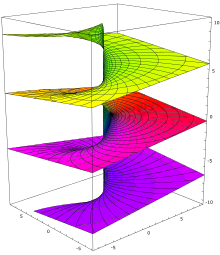
\includegraphics[width = .6\textwidth]{logz}
	\caption{The complex logarithm with multiple branches.}
\end{figure}
The function forms a spiral around 0; as we wrap around 0, the logarithm gets larger. This can be seen intuitively because 
as $d\log(z)/dz = 1/z$, so if we want to evaluate the change in the logarithm from $z_2$ to $z_1$, we can integrate $1/z$ like 
so:
\begin{equation}
	\log(z_1) - \log(z_2) = \int_{z_2}^{z_1}\frac{dz}{z}
\end{equation}
But, notice that this does not specify the path we are taking. Namely, we can take a closed loop $C$ around the origin, 
parameterized by $C = \{\cos(t) + i\sin(t) : t\in [0, 2\pi]\}$, to evaluate this integral. Starting this integral at $z_1 = z_2 = 1$, we 
plug in $z = \cos(t) + i\sin(t)$ to see:
\begin{equation}
	\log(1_+) - \log(1_-) = \oint_C \frac{dz}{z} = \int_0^{2\pi}dt\frac{-sin(t) + i\cos(t)}{\cos(t) + i\sin(t)} = \int_0^{2\pi} 
	dt\frac{i(\sin^2(t) +\cos^2(t))}{\cos^2(t) + \sin^2(t)} = 2\pi i~
	\label{eq:oneoverz}
\end{equation}
which is non-zero. As we wrap around 0, the value of the function $\log(z)$ can change: it is multiple valued, and there is 
nothing saying we cannot get to another possible value for $\log(1)$ if we move along a curve surrounding the origin. 

To make this more precise, we choose a branch by \textit{defining} the value of $\log(z_0)$ for some $z_0\in\mathbb C$ as 
one of its possible values. Consider defining 
$\log((r + \epsilon) e^{i\theta})$ for $\epsilon$ infinitesimal. The possible values of this we can choose from are 
$\log(r + \epsilon) + i\theta + 2\pi i n$ for $n\in\mathbb Z$, but here's the key point: only one specific value of $n$ works if 
we want this definition of the logarithm to be continuous! In this way, we can build up the definition of the logarithm on this 
branch (this is called the \textbf{principal branch} of the logarithm) until we have defined it on almost the entire complex plane. 

Branch cuts come in when we have defined the logarithm almost everywhere. We \textit{cannot} wrap the logarithm around the 
entire plane, or else we will have to deal with the fact that it is multi-valued when we wrap around the origin. We can extend it 
almost everywhere, but there must be at least a ray in the complex plane starting from 0 for where we cannot define $\log(z)$, 
or else we could continue this ``wrapping around 0" nonsense and destroy the single-valuedness of our branch. 

 can extend $\log(z)$ by integrating its derivative $\frac{1}{z}$. We


\subsection{Analytic Continuation}

Analytic continuation is perhaps one

\subsection{Laurent Series}

\subsection{Example: Wick rotation}

The canonical example of this that you've likely seen in a physics class is a \textbf{Wick rotation} in which time $t$ is replaced 
with imaginary time $\tau$ via:
\begin{equation}
	t\mapsto i\tau
\end{equation}
This exact example occurs as well in the correspondence between statistical mechanics and quantum mechanics, as the 
replacement $t\mapsto i\beta$ maps time evolution to the statistical Boltzmann factor:
\begin{equation}
	e^{iHt}\mapsto e^{-\beta E}
\end{equation}
where we identify $H$ with $E$.

In Minkowski spacetime, the advantage of a Wick rotation is apparent when one considers the metric:
\begin{equation}
	ds^2 = dt^2 - d\vec x^2 = (id\tau)^2 - d\vec x^2 = -(d\tau^2 + \vec d\vec x^2)
\end{equation}
After Wick rotation, the Minkowski metric becomes Euclidean. This means that if we have an integral over Minkowski 
spacetime, Wick rotation takes this into an ordinary Euclidean space integral and we can use all the formulas we know and 
love. Note the measure $d^4 k = dk_t\, d\vec k = i dk_\tau\, d\vec k = d^4 k_E$ where $k_E$ is the Euclidean momenta, and 
the invariant square $k^2 = k_t^2 - \vec k^2 = (ik_\tau)^2 - \vec k^2 = -k_E^2$, so for example:
\begin{equation}
	\int \frac{d^4 k}{k^2} = \int\frac{id^4 k_E}{-k_E^2} = -\int d\Omega_3 \int dk_E\, \frac{k_E^3}{k_E^2} = - \Omega_3 
	\int dk_E\, k_E
\end{equation}
where $\Omega_3$ is the measure on the shell $S^3$ (this is in contrast to $d^3\vec k = k^2\,dk\, d\Omega_2 = d^2\,dk\, 
\sin\theta\,d\theta\,d\phi$ in 3 dimensional space, since $k_E$ is a four dimensional Euclidean vector). 

We are discussing Wick rotation because when asked when it works, the usual response by a physicist is to simply say 
``analytic continuation!" and move on. In fact, analytic continuation is a rather small part of why the Wick rotation works. 

\end{document}